% !TEX encoding = UTF-8
% !TEX TS-program = pdflatex
% !TEX root = ../tesi.tex

%**************************************************************
\chapter{Resoconto dello stage}
\label{cap:resoconto-stage}
%**************************************************************

\intro{In questo capitolo verranno descritte le attività svolte durante lo stage. Per ogni attività si cercherà di descrivere il problema affrontato, le scelte effettuate ed i test svolti.}\\

\section{Pianificazione}
La prima attività svolta, in realtà ancora prima dell'inizio dello stage stesso, è stata quella di pianificare il lavoro da svolgere. Tale pianificazione è stata concordata tra il tutor aziendale e il sottoscritto, ed è esposta nella sezione \ref{sec:vincoli-temporali} a pagina \pageref{sec:vincoli-temporali} di questo documento.\\
Tale pianificazione, però, è stata "aggiustata" (ma mai stravolta) in base a quanto svolto settimana per settimana, decidendo di dedicare più o meno ore ad una determinata attività.\\
Al termine di ogni settimana, periodo coincidente con il raggiungimento di un obiettivo, infine, è stato deciso che avrei dovuto redarre una breve relazione, con lo scopo di documentare il lavoro svolto. Tali relazioni, inoltre, sono servite come materiale ausiliario per la presentazione delle nuove funzionalità sviluppate al proponente. Infine, terminati tutti gli obiettivi e in caso di approvazione da parte del tutor e del proponente, avrei dovuto trasferire il lavoro svolto dall'ambiente di sviluppo a quello di produzione.

\section{Studio del funzionamento del Booking Engine}

\subsection{OTA e DataExchange}
Appena iniziato lo stage, mi sono subito dedicato all'analisi della struttura di CrociereRegalo, grazie anche (soprattutto all'inizio) all'aiuto del mio tutor. Come prima cosa, mi è stato spiegato che il Booking Engine, in realtà, era spezzato in due parti dipendenti l'una dall'altra: \textbf{OTA} (disponibile all'indirizzo \url{https://www.crociereregalo.it}) e \textbf{DataExchange} (disponibile all'indirizzo \url{https://data.crociereregalo.it}). L'idea alla base di questa divisione è che la parte \textit{OTA} rappresenti il sito web vero e proprio, con il quale l'internauta si affaccia, mentre la parte \textit{DataExchange} serva per l'interazione tra \textit{OTA} e \glspl{webservice} dei vari fornitori (dove per fornitori si intendono le varie compagnie di crociera). 

\subsection{Interazione tra OTA e DataExchange}
\textit{OTA} e \textit{DataExchange} sono sì dipendenti l'uno dall'altro, ma hanno due database separati. Questo, fondamentalmente, avviene perchè i dati provenienti da i vari fornitori hanno formati diversi, che devono quindi essere uniformati per poter essere processati secondo una logica più indipendente possibile. Il compito del \textit{DataExchange} è proprio questo: interrogare i \glspl{webservice} dei vari fornitori, ricevere i dati, elaborarli, uniformarli e passarli ad \textit{OTA}.\\
Premesso ciò, vi sono due possibili interazioni tra \textit{OTA} e \textit{DataExchange}
\begin{itemize}
	\item Interazione \textbf{schedulata}, che avviene circa 3 volte al giorno, il cui compito è sincronizzare i cataloghi (chiamati anche \textit{flatfile}) dei vari fornitori per rendere disponibili le (eventuali) modifiche alla parte \textit{OTA} del Booking Engine. \\Quando un visitatore del sito CrociereRegalo cerca una crociera, tale ricerca avviene interrogando i cataloghi presenti nel database della parte \textit{OTA}, senza quindi interrogare i \glspl{webservice} delle compagnie di crociera (per motivi di prestazione dovuti all'ingente mole di dati da elaborare). I cataloghi, quindi, vengono scaricati nel DataExchange, elaborati (uniformati) e poi sincronizzati con il database di OTA; la procedura di sincronizzazione viene chiamata \textbf{Integrazione}. L'integrazione avviene attraverso l'invocazione (grazie allo scheduler di \textit{Windows Server}) che, grazie ad una chiamata \textit{HTTP} ad una particolare pagina del DataExchange, invoca la procedura di integrazione dati.
	\begin{figure}[!h] 
		\centering 
		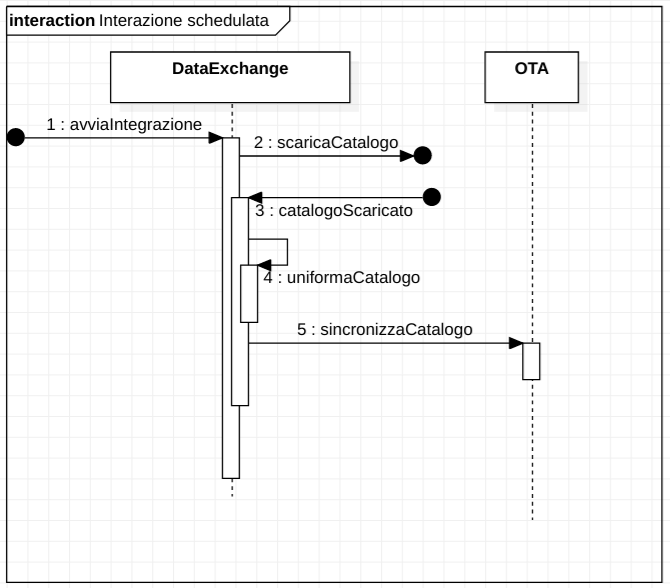
\includegraphics[width=0.8\columnwidth]{attivita/interazione_schedulata} 
		\caption{Schema dell'integrazione schedulata appena descritta.}
	\end{figure}
	\item Interazione \textbf{real-time}, che avviene durante tutto il flusso di prenotazione di una cabina (che analizzerò in seguito). Tale flusso deve per forza disporre di dati aggiornati in tempo reale, altrimenti potrebbero verificarsi problemi in fase di prenotazione (come la prenotazione di una cabina non più disponibile). L'interazione in tempo reale avviene attraverso delle chiamate \textit{HTTP} (ajax) effettuate nel momento del bisogno dall'\textit{OTA} al \textit{DataExchange}, attraverso lo scambio di dati in formato \textit{JSON}.
	\begin{figure}[!h] 
		\centering 
		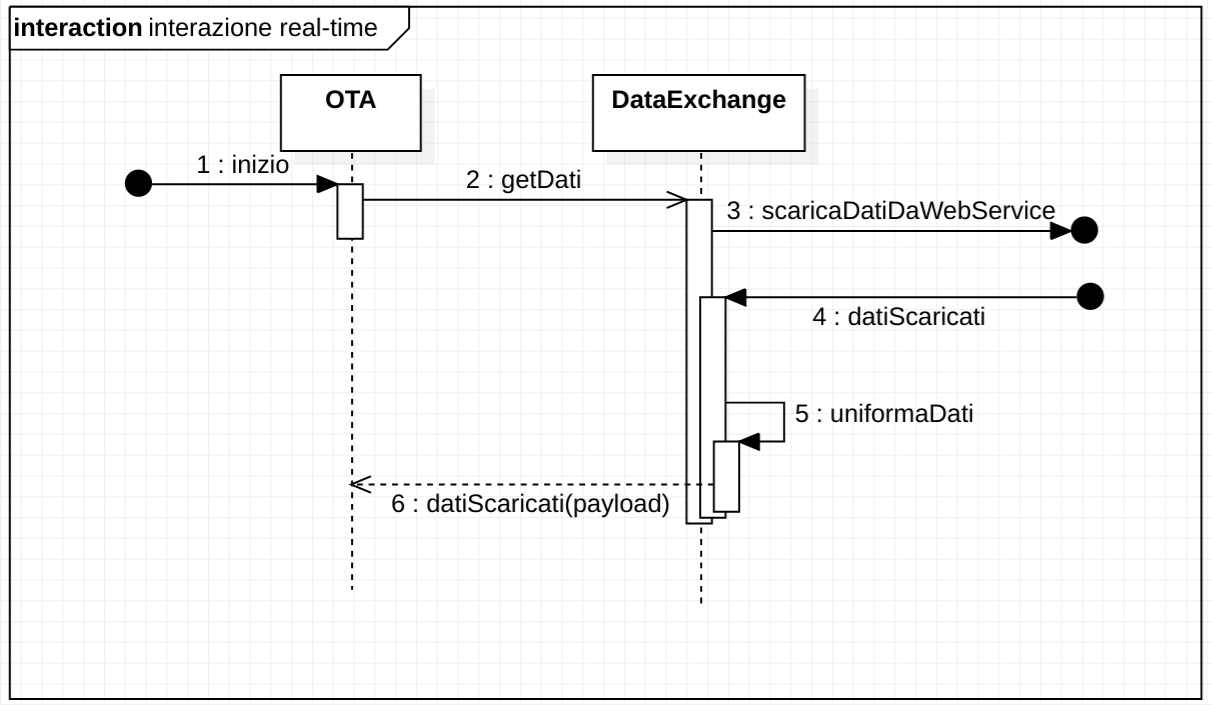
\includegraphics[width=0.8\columnwidth]{attivita/interazione_realtime} 
		\caption{Schema dell'integrazione in tempo reale appena descritta.}
	\end{figure}
\end{itemize}